\documentclass{article}
\usepackage[utf8x]{inputenc}
\usepackage{ucs}
\usepackage{amsmath} 
\usepackage{mathtext}
\usepackage{amsfonts}
\usepackage{upgreek}
\usepackage[english,russian]{babel}
\usepackage{graphicx}
\usepackage{float}
\usepackage{textcomp}
\usepackage{hyperref}
\usepackage{geometry}
  \geometry{left=2cm}
  \geometry{right=1.5cm}
  \geometry{top=1cm}
  \geometry{bottom=2cm}
\usepackage{tikz}
\usepackage{ccaption}
\usepackage{multicol}
%\setlength{\columnsep}{1.5cm}
%\setlength{\columnseprule}{0.2pt}


\begin{document}
\pagenumbering{gobble}


\section*{Домашнее задание}
\subsection*{Очередь}
\begin{multicols}{2}
\begin{verbatim}
#define CAPACITY 7
typedef int Data;

struct queue
{
    int front;
    int back;
    Data values[CAPACITY];
};
typedef struct queue Queue;

// ......

int main()
{
    Queue a;
    a.init();
    enqueue(&a, 100);
    for (int i = 0; i < 20; ++i)
    {
        enqueue(&a, i);
        dequeue(&a);
    }
    enqueue(&a, 200);
    print_queue(&a);
}
\end{verbatim}
Очередь — абстрактный тип данных с дисциплиной доступа к элементам «первый пришёл — первый вышел». \\
Реализация с помощью массива:

\begin{center}
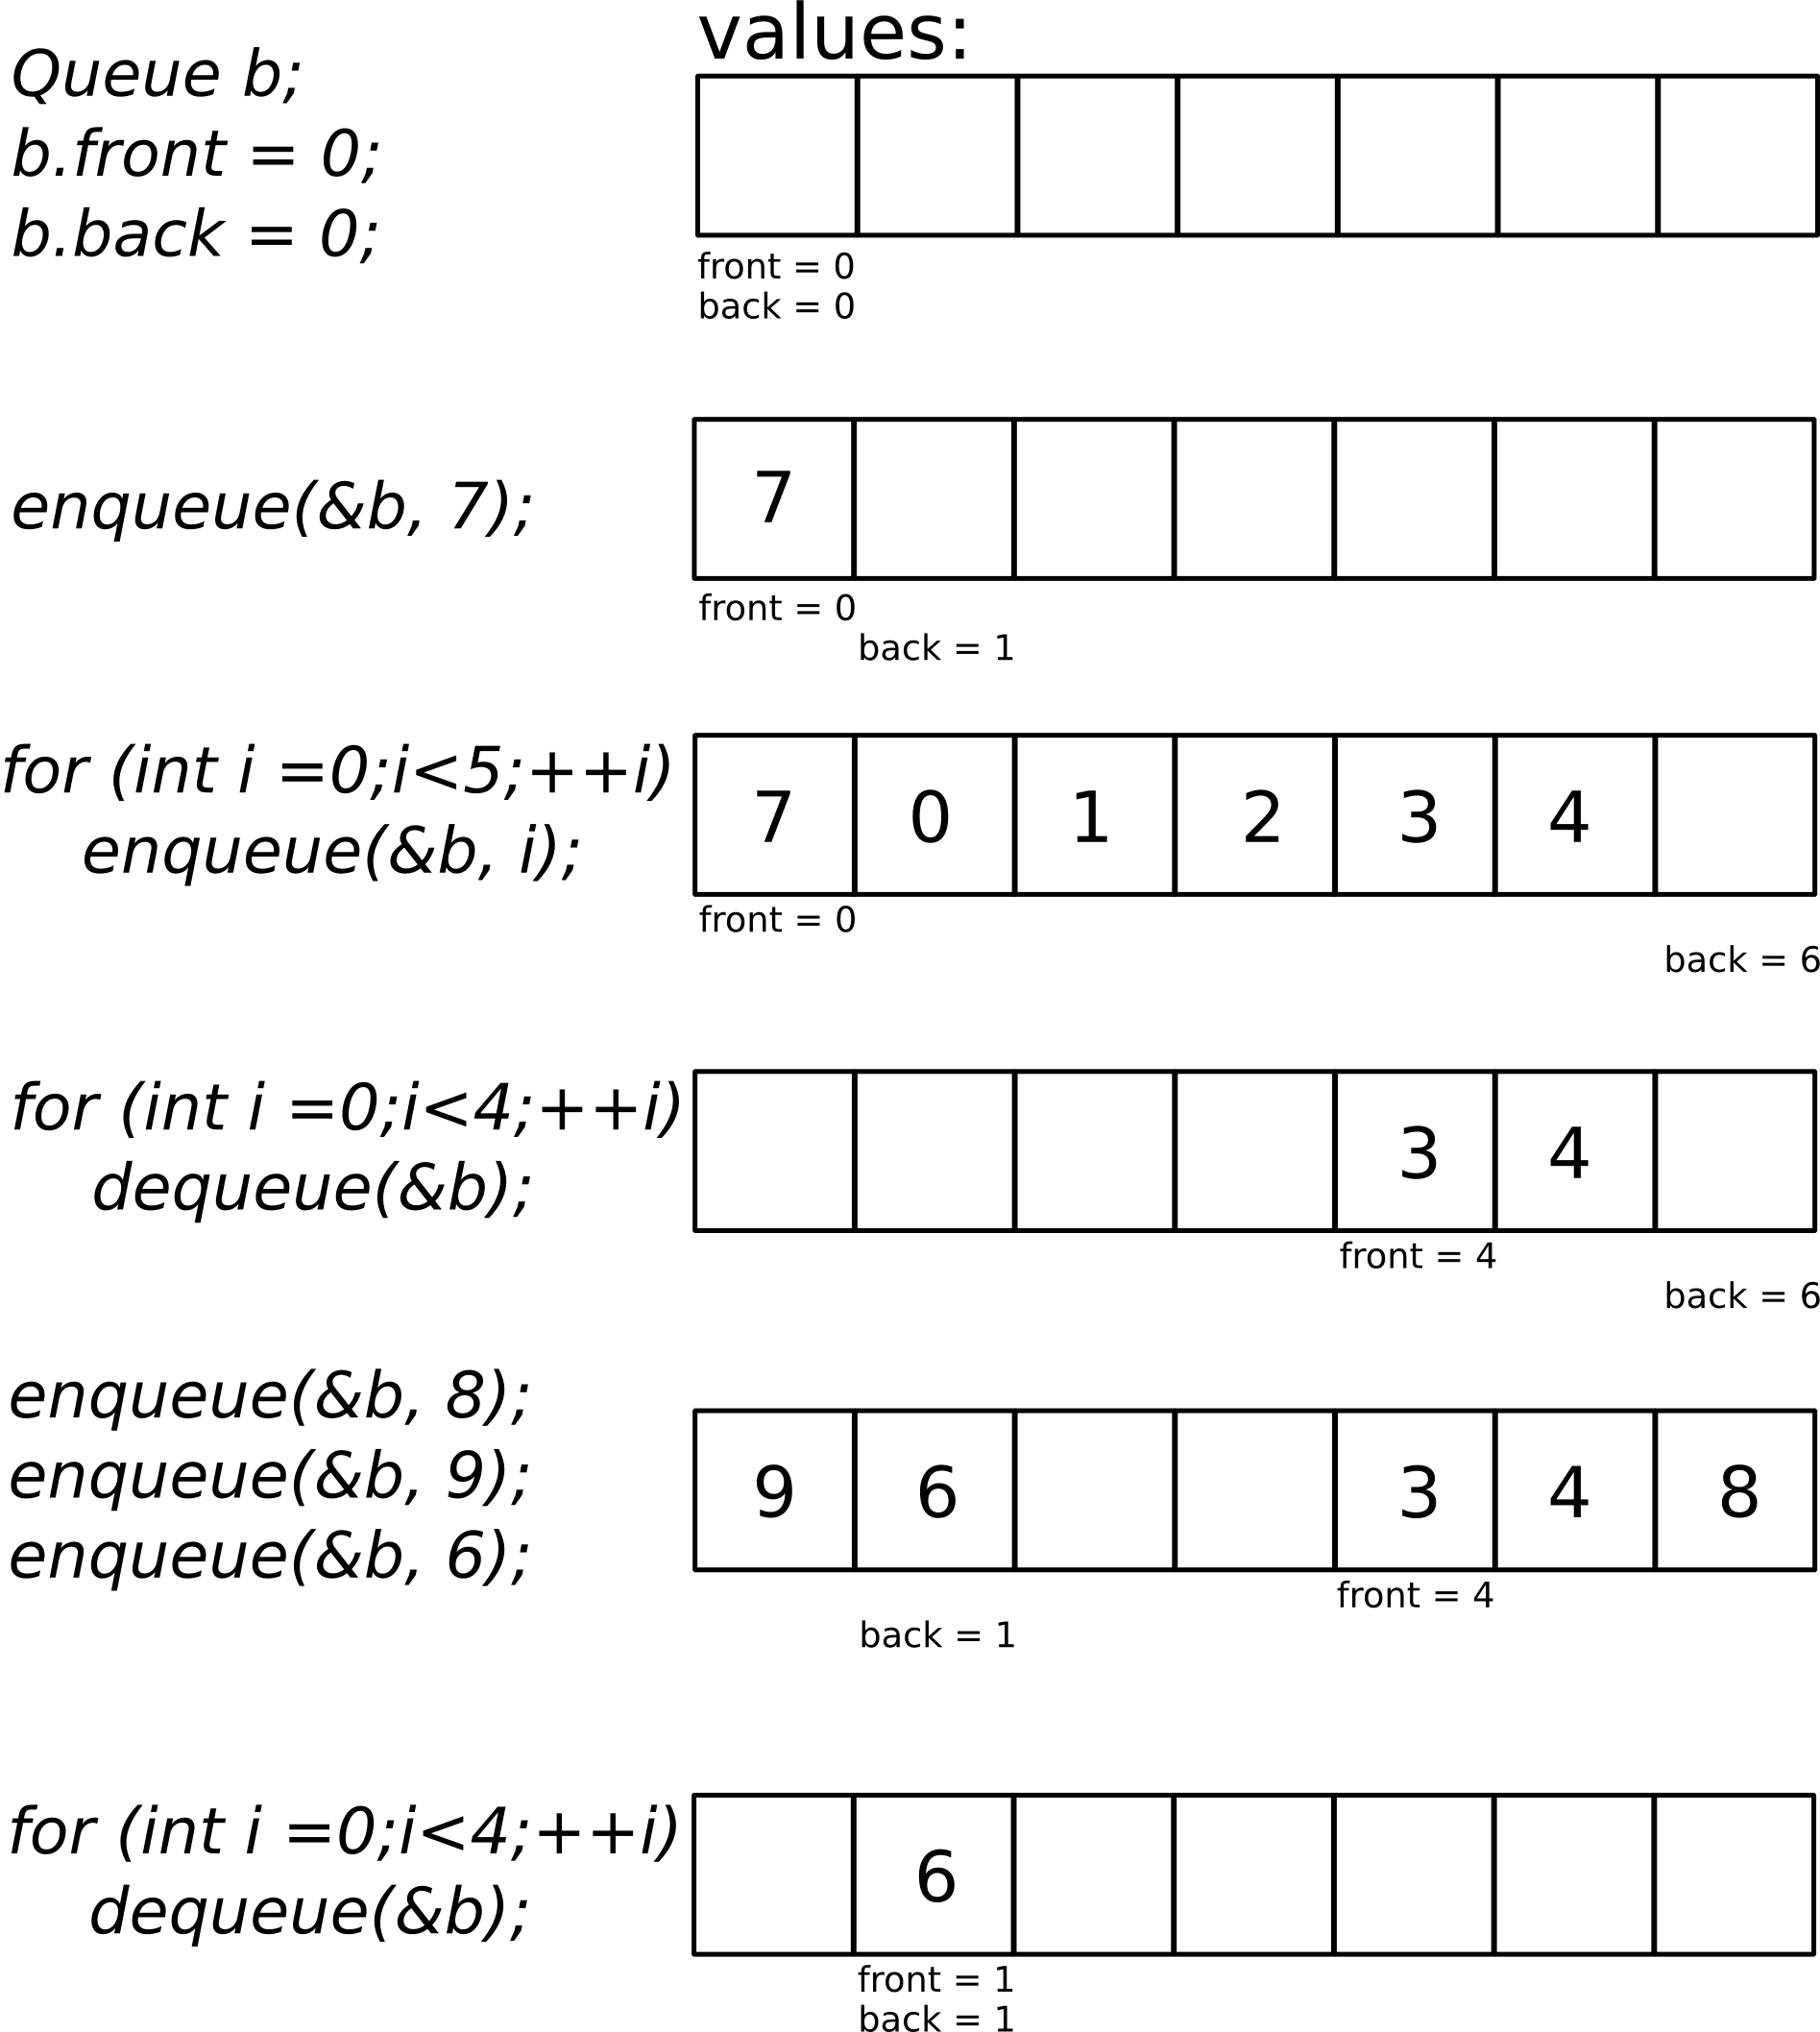
\includegraphics[width=0.95\linewidth]{../images/queue.png}
\end{center}
\end{multicols}

\subsubsection*{Очередь со статическим массивом. Задачи:}
\begin{enumerate}
\item Написать функцию \texttt{void enqueue(Queue* q, Data x)}.
\item Написать функцию \texttt{Data dequeue(Queue* q)}.
\item Написать функцию \texttt{void queue\_init(Queue* q)}.
 Протестируйте очередь: проверьте, что выведет программа, написанная выше.
\item Написать функцию \texttt{int queue\_is\_empty(Queue* q)}, которая возвращает 1 если очередь пуста и 0 иначе.
\item Написать функцию \texttt{int queue\_get\_size(Queue* q)}, которая возвращает число элементов в очереди (не capacity!).
\item Написать функцию \texttt{int queue\_is\_full(Queue* q)}, которая возвращает 1 если очередь заполнена и 0 иначе.
\item Написать функции \texttt{Data queue\_get\_front(Queue* s)} и \texttt{Data queue\_get\_back(Queue* s)}, которые возвращают элементы, находящиеся в начале и в конце очереди соответственно, но не изменяют очередь.
\item Написать функцию \texttt{void queue\_print(Queue* s)}, которая распечатывает все элементы очереди.
\item Что произойдёт, если вызвать enqueue() при полной очереди или dequeue() при пустой? Обработайте эти ситуации. Программа должна печатать сообщение об ошибке и завершаться с аварийным кодом завершения. Чтобы завершить программу таким образом можно использовать функцию exit() из библиотеки stdlib.h. Пример вызова: exit(1);

\item Протестируйте очередь на следующих тестах:
\begin{enumerate}
\item В очередь добавляется 4 элемента, затем удаляется 2. Вывести содержимое очереди с помощью \texttt{queue\_print()}
\item В очередь добавляется очень много элементов (больше чем CAPACITY). Программа должна напечатать сообщение об ошибке.
\item В очередь добавляется 3 элемента, затем удаляется 2, затем очень много элементов (больше чем CAPACITY). Программа должна напечатать сообщение об ошибке.
\item В очередь добавляется 3 элемента, затем удаляется 4. Программа должна напечатать сообщение об ошибке.
\item В очередь добавляется 2 элемента, затем выполняется следующий цикл:
\begin{verbatim}
for (int i = 0; i < 10000; ++i)
{
    enqueue(&a, i);
    dequeue(&a);
}
\end{verbatim}
Вывести содержимое очереди с помощью \texttt{queue\_print()}
\end{enumerate}

\subsubsection*{Очередь с динамическим массивом. Задачи:}

Описание такой очереди выглядит следующим образом:
\begin{verbatim}
struct queue
{
    int capacity;
    int front;
    int back;
    Data* values;
};
typedef struct queue Queue;
\end{verbatim}

\item Скопируйте код очереди со статическим массивом в новый файл и измените описание структуры как показано выше. Define-макрос CAPACITY больше не нужен, его можно удалить.

\item Измените функцию \texttt{void queue\_init(Queue* q)} на \texttt{void queue\_init(Queue* q, int initial\_capacity)}. Теперь она должна присваивать capacity начальное значение initial\_capacity и выделять необходимую память под массив values.

\item Измените функцию \texttt{void enqueue(Queue* q)}. Теперь, при заполнении очереди должно происходить перевыделение памяти с помощью функции realloc(). После перевыделения нужно переместить элементы массива на новые места и изменить front и back. Если front != 0, то нужно переместить элементы массива от front до конца старого массива values в конец нового массива values.

\item Добавьте функцию \texttt{void queue\_destroy(Queue* q)}, которая будет освобождать память, выделенную под массив values.

\item Протестируйте очередь: в очередь добавляется очень много элементов (> 1000 > initial\_capacity). Программа \textbf{не} должна напечатать сообщение об ошибке.
\end{enumerate}

\end{document}